\section{Related Works}
\label{sec:relatedworks}
WSNs have become an increasingly compelling platform for SHM applications due to the advantages in low cost, easy of deployment and flexibility compared with the wire-based counterparts\cite{jeongyeup2005embedded}. WSNs also permit a much higher spatial density of sensors over existing wired network, thus potentially increases the SHM quality that can be achieved.

Modal analysis has been widely used in SHM. From deployed sensors, the vibration characteristics (i.e. modal parameters) of the structures are identified using modal analysis.  Modal parameters are the internal properties of a structure and can be used to detect and locate possible structural damage. 

So far, WSN-based SHM systems which implement modal analysis generally have two types of architectures: centralized and distributed.  A typical centralized architecture is illustrated in Fig. \ref{fig:ModalArchitectures}a.  Systems of this architecture are intrinsically equivalent to wire-based counterpart \cite{kim2007health}. In these systems, measurements collected by each sensor node are wirelessly transmitted to a central unit where modal analysis is implemented to obtain the modal parameters of the whole structure. Classic modal identification algorithms such as the eigen realization algorithm (ERA) \cite{juang1985eigensystem}, the subspace algorithm (SS)\cite{ljung1987system}, etc., can be directly used without any modification. However, systems of this architecture have poor scalability and relatively high energy consumptions. 

\begin{figure}
\centering
%\figurecurrentwidth{modalcluster-resized}
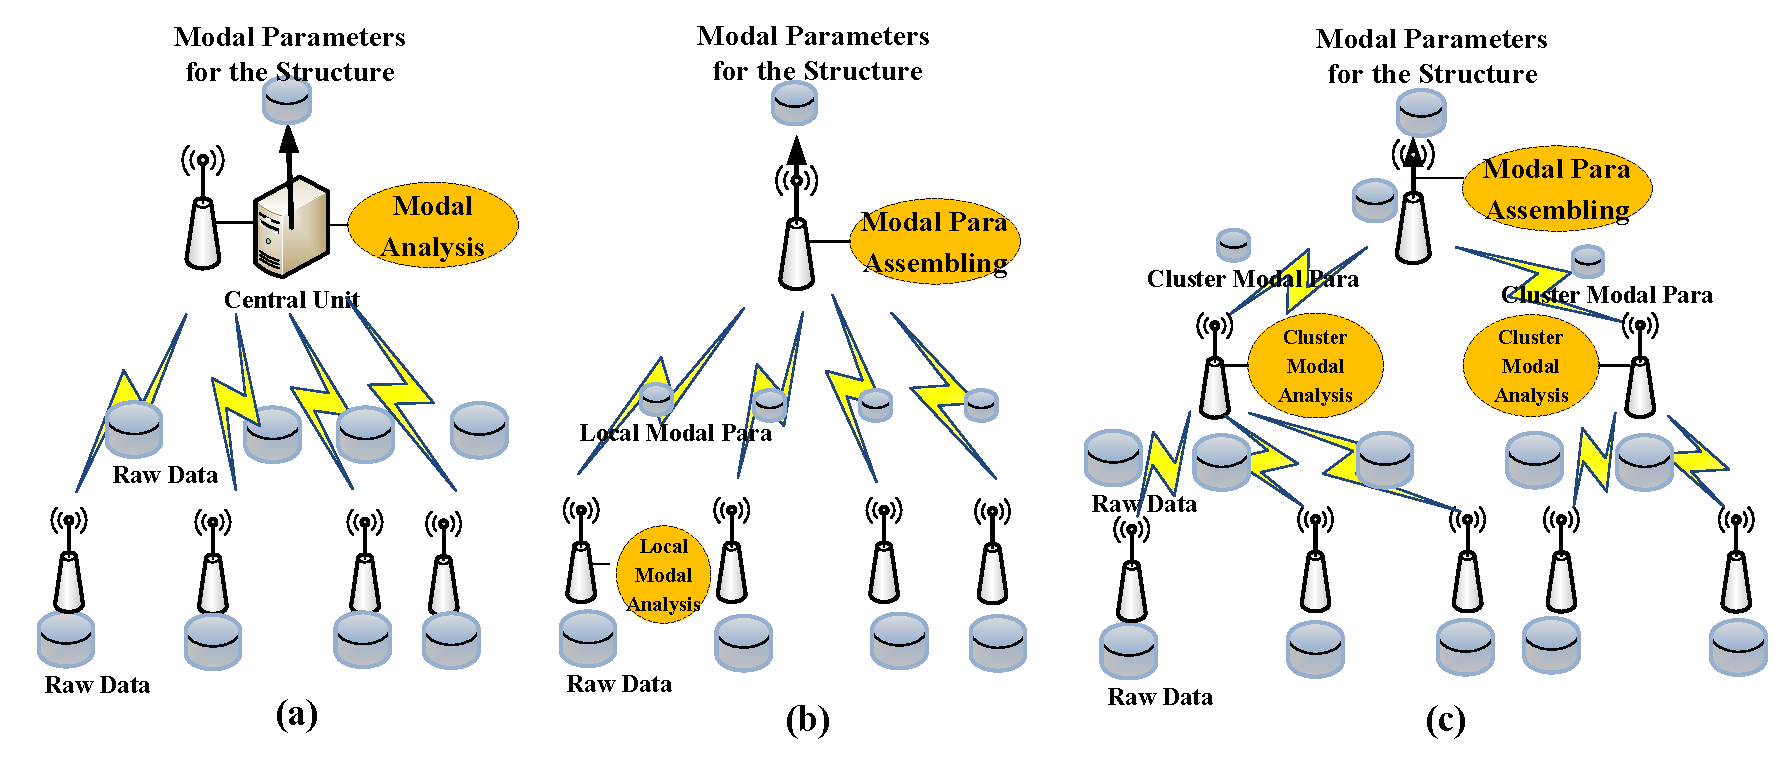
\includegraphics[width=.45\textwidth,height=.22\textwidth]{ModalArchitectures}%, height=.5\textwidth]
\caption{Three WSN architectures for modal analysis, (a) Centralized (b) Distributed (c) Cluster-based}
\label{fig:ModalArchitectures}
\end{figure}
To address the aforementioned problems, civil researchers have proposed a method to implement modal analysis in a fully distributed way. The system architecture is illustrated in Fig. \ref{fig:ModalArchitectures}b. In this method, each sensor node implements modal analysis based on simple peak-picking technique \cite{ewins1984modal}. The modal parameters identified from each sensor node are then transmitted to a central unit, where these modal parameters are assembled together.  The particular advantage of these systems is energy efficiency: local modal analysis is made without data exchange and transmitting only the modal parameters requires much less energy than streaming the raw data. However, since each sensor node in this approach performs modal analysis based on its own measured data without any collaboration with others, input change or measurement noise can easily degrade the identified local modal parameters and the errors cannot be reduced in the assembling process at the central unit.

In this paper, to address the problems of both architectures above, we proposed a cluster-based approach for modal analysis in SHM. This architecture is presented in Fig. \ref{fig:ModalArchitectures}c.  In this approach, the whole network is partitioned into a number of single-hop clusters. A cluster head (CH) is designated in each cluster to perform intra-cluster modal analysis using traditional centralized modal identification algorithms. The identified modal parameters in each cluster are then assembled together to obtain the modal parameters for the whole structure. Compared with the centralized approach, the cluster-based modal analysis limits the number of sensor nodes and hop count in each cluster, thus can be more energy efficient and scalable. Compared with the distributed approach, classic modal parameter identification techniques which use data-level fusion can be used in each cluster to obtain more reliable and accurate results. This cluster-based approach is therefore suitable for WSN-based SHM systems. In this approach, how to partition sensor nodes is critical. Clustering should address requirements from both modal analysis and wireless sensor networks (particularly in terms of energy). This optimal clustering problem is the focus of this paper.

Strictly speaking, a work proposed in \cite{zimmerman2008automated} can be regarded as a simplified cluster-based modal analysis where each cluster contains exact two sensor nodes. However, the authors did not consider other topologies and the problem of how to optimize clustering to decrease energy consumption of WSNs. Also, the paper assumes all the sensor nodes are in a single communication range. 

%\begin{figure}
%\centering
%\subfloat[]{\label{fig:cluster1}
%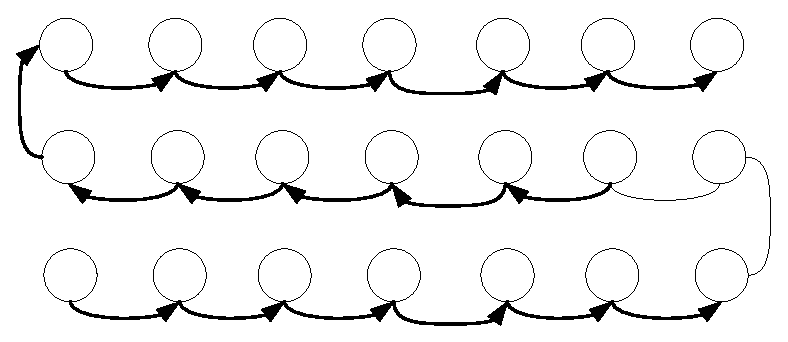
\includegraphics[width=.15\textwidth]{cluster1}}
%\subfloat[]{\label{fig:cluster2}
%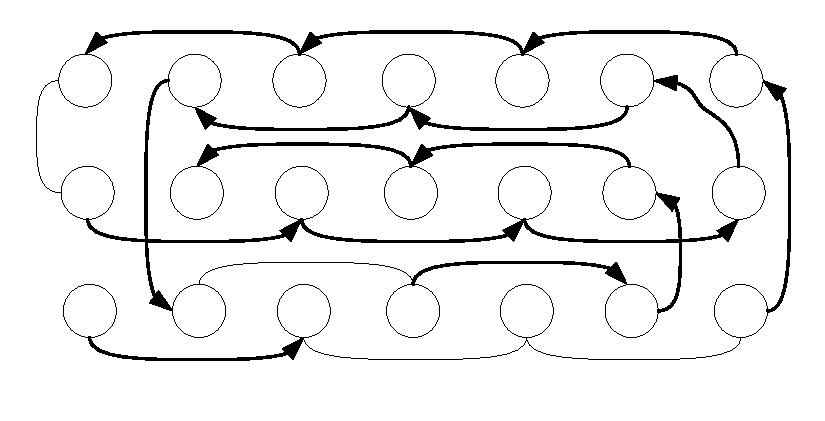
\includegraphics[width=.15\textwidth]{cluster2}}
%\subfloat[]{\label{fig:cluster3}
%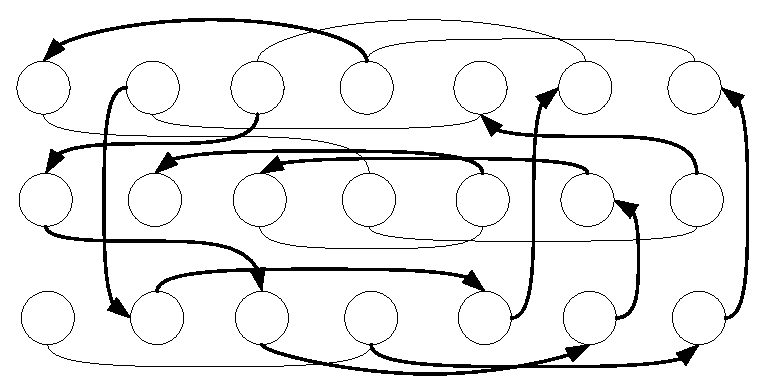
\includegraphics[width=.15\textwidth]{cluster3}}
%\caption{Three proposed architectures by civil researchers [ref]}
%\label{fig:clustering}
%\end{figure}

Clustering has been exhaustively studied by researchers in computer science engineering and has been used in many applications to improve system performance, particularly in terms of local resources arbitration (e.g. in MAC protocol) and system scalability.  Many clustering algorithms, such as LEACH \cite{leach},HEED \cite{iheed}, have been proposed. However, we will show in the following sections our clustering problem has some particular requirements from modal analysis and the existing clustering algorithms cannot be directly applied.